\textbf{Определение.} \textbf{Нормальной системой} дифференциальных уравнений порядка $n$ называется система уравнений вида
\begin{equation*}
    \begin{cases}
    \dot{x}_1 = f_1(t, x_1,\ldots,x_n)\\
    \ldots\\
    \dot{x}_n = f_n(t, x_1, \ldots, x_n)
    \end{cases}
\end{equation*}

Если ввести в рассмотрение векторы
\begin{equation*}
    r = \begin{pmatrix}
    x_1\\
    \ldots\\
    x_n
    \end{pmatrix}, \quad
    f(t,r) = \begin{pmatrix}
        f_1(t,r)\\
        \ldots\\
        f_n(t,r)
    \end{pmatrix}
\end{equation*}
то систему можно компактно записать в виде одного $n$-мерного уравнения
\begin{equation}
    \dot{r} = f(t,r) \label{normsyst}
\end{equation}

\noindent \textbf{Определение.} Вектор-функция $\varphi$ --- \textbf{решение системы} (\ref{normsyst}), если
\begin{itemize}
    \item $\varphi \in C^1((a,b) \to \mathbb{R}^n)$
    \item $\dot{\varphi}(t) \equiv f(t, \varphi(t))$ на $(a,b)$
\end{itemize}

\noindent \textbf{Определение.} \textbf{Задачей Коши} для системы (\ref{normsyst}) называется задача нахождения ее решения, удовлетворяющего начальному условию $r(t_0) = r_0$.\\

\noindent \textbf{Лемма (О равносильном интегральном уравнении.)} Пусть $t_0 \in [a,b]$, $G \subset \mathbb{R}^{n + 1}$ --- область, $(t_0, r_0) \in G$, $f \in C(G \to \mathbb{R}^n)$. Тогда $\varphi$ --- решение на $[a,b]$ задачи Коши.
\begin{equation}
    \dot{r} = f(t,r), \quad r(t_0)=r_0 \label{zksyst}
\end{equation}
если и только если $\varphi$ --- решение на $[a,b]$ уравнения
\begin{equation}
    r(t) = r_0 + \int_{t_0}^{t} f(\tau, r(\tau))d\tau \label{inteq}
\end{equation}
\textbf{Доказательство.} Пусть $\varphi$ --- решение (\ref{zksyst}) на $[a,b]$. Тогда $\varphi \in C[a,b]$. Интегрируя равенство $\dot{\varphi}(\tau) = f(\tau, \varphi(\tau))$ от $t_0$ до $t \in [a,b]$, имеем
\begin{equation*}
    \varphi(t) - \varphi(t_0) = \int_{t_0}^{t} f(\tau, \varphi(\tau))d\tau
\end{equation*}
Поскольку $\varphi(t_0) = r_0$, то функция $\varphi$ --- решение уравнения (\ref{inteq}) по определению.

Докажем обратное. Пусть $\varphi$ --- решение (\ref{inteq}) на $[a,b]$. Тогда из равенства
\begin{equation}
    \varphi(t) = r_0 + \int_{t_0}^{t} f(\tau, \varphi(\tau))d\tau \label{phieq}
\end{equation}
следует, что $\varphi \in C^1[a,b]$. Дифференцируя (\ref{phieq}) по $t$, получаем $\dot{\varphi} \equiv f(t, \varphi(t))$ на $[a,b]$. Кроме того, из (\ref{phieq}) вытекает $\varphi(t_0) = r_0$. Таким образом, $\varphi$ --- решение (\ref{zksyst}) по определению.\\

\noindent \textbf{Определение.} Пусть $G \subset \mathbb{R}_{t,r}^{n+1}$ --- область, $(t_0, r_0) \in G$. Поскольку $G$ --- открытое множество, то найдутся числа $a,b > 0$, такие что параллелепипед
\begin{equation*}
    \Pi = \left\{(t,r) \in \mathbb{R}^{n+1}\,|\, |t-t_0| \le a, |r-r_0|\le b \right\}
\end{equation*}
целиком содержится в области $G$. Так как $\Pi$ --- компакт, то существует число $M = \displaystyle\max_{(t,r)\in \Pi} |f(t,r)|$. Положим $h = \min \{a, \frac{b}{M}\}$ (если $M = 0$, то $h = a$). Отрезок $[t_0 - h, t_0 + h]$ называется \textbf{отрезком Пеано}, соответсвующим точке $(t_0, r_0)$ (см. \hyperref[peano]{рисунок}).

Отрезок Пеано, таким образом, определен неоднозначно. Зафиксируем один из них и разобъем его правую половину на $N \in \mathbb{N}$ равных частей точками
\begin{equation*}
    t_k = t_0 + \frac{kh}{N}, \quad k \in [1 : N]
\end{equation*}
Определим ломаную Эйлера $E_N$: $[t_0, t_0 + h] \to \mathbb{R}$ рекуррентно:
\begin{equation}
    \begin{aligned}
        &E_N(t_0) = r_0,\\
        &E_N(t) = E_N(t_k) + f(t_k, E_N(t_k))(t - t_k), \text{ если } t \in (t_k, t_{k+1}]
        \label{eulerlom}
    \end{aligned}
\end{equation}

Если $(t_k, E_N(t_k)) \notin G$ при некотором $k$, то функция $E_N$ не может быть определена на всем промежутке $[t_0, t_0 + h]$. Следующая лемма показывает, что такая ситуация исключена.\\

\noindent \textbf{Лемма (свойства ломаной Эйлера).} Для любого $t \in [t_0, t_0 + h]$
\begin{enumerate}
    \item функция $E_N$ определена в точке $t$
    \item $|E_N(t) - r_0| \le M(t - t_0)$
\end{enumerate}
\textbf{Доказательство.} Методом математической индукции установим, что утверждения (1) и (2) верны при $t \in [t_0, t_k]$ для любого $k \in [1 : N]$.

При $k = 1$ функция $E_N$ определена на $[t_0, t_1]$. Имеем
\begin{equation*}
    |E_N(t) - r_0| = |r_0 + f(t_0, r_0)(t - t_0) - r_0| = |f(t_0, r_0)|(t - t_0) \le M(t - t_0)
\end{equation*}
\begin{figure}[h!]\label{peano}
    \center{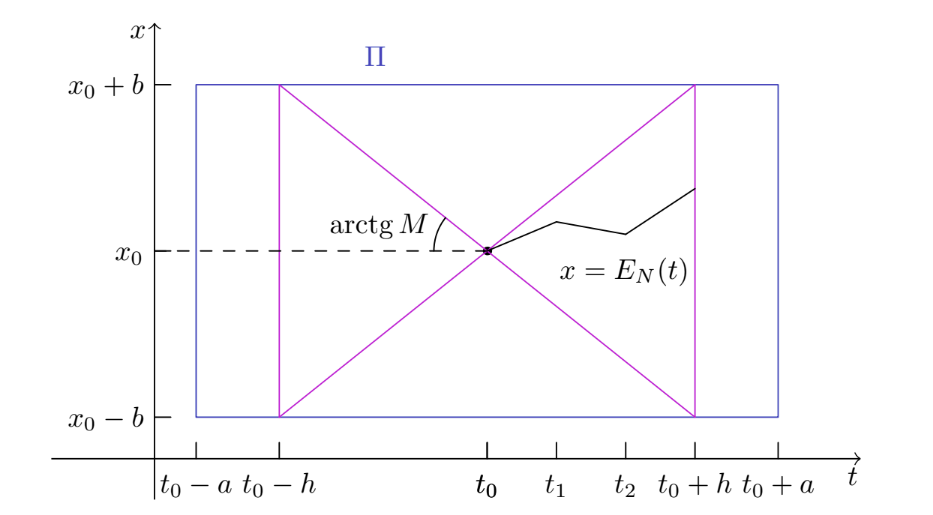
\includegraphics[scale=0.5]{Pics/Screenshot from 2021-01-14 22-03-34.png}}
\end{figure}

Допустим, что утверждения (1) и (2) установлены для $t \in [t_0, t_k]$ при некотором $k \in [1 : N - 1]$. Из пункта (2) тогда следует
\begin{equation*}
    |E_N(t_k) - r_0| \le M(t_k - t_0) \le Mh \le M \frac{b}{M} = b
\end{equation*}
то есть $(t_k, E_N(t_k)) \in \Pi$, а значит $E_N$ можно определить на $[t_k, t_{k+1}]$.

Проверим (2) при $t \in (t_k, t_{k+1}]$:
\begin{equation*}
    \begin{aligned}
        &|E_N(t) - E_N(t_0)| \le |E_N(t) - E_N(t_k)| + |E_N(t_k) - E_N(t_0)| \le\\
        &\le |f(t_k, E_N(t_k))|(t-t_k) + M(t_k - t_0) \le M(t - t_k) + M(t_k - t_0) = M(t - t_0)
    \end{aligned}
\end{equation*}
